%% ma: L10-B24-0002
%% lop: 10
%% chuong: 8
%% bai: 24
%% dang: 10.24.1
%% loai: TLN
%% muc: VD
%% dap_an: "35"
%% nguon: "(NBV)-ĐỀ SỐ 1-MỖI NGÀY 1 ĐỀ THI 2025.pdf (D01, MỖI NGÀY 1 ĐỀ - Đề số 1), Phần III Câu 2"
%% kien_thuc: "Đồ thị có trọng số, chu trình Hamilton (không có trong mục lục sgk-kntt.yaml); cách giải liệt kê hoán vị (Lớp 10 Bài 24, vị trí tạm đã được giáo viên duyệt cho dạng 10.24.1)"
%% ghi_chu: "Hình dựng lại từ hình gốc (10 cạnh đủ trọng số). Lời giải gốc dùng thuật toán láng giềng gần nhất (chỉ là heuristic, không bảo đảm tối ưu); đã liệt kê đủ 12 chu trình và xác nhận min = 35, đáp án gốc 35 đúng. So với L10-B24-0001: đồ thị 5 đỉnh (12 chu trình) thay vì 4 đỉnh nên coi là không trùng"
%% trang_thai: chinh-thuc
\begin{ex}
Từ kho $D$, xe bưu chính đến lấy thư từ các hộp thư tại $E,F,G$ và $H$ rồi quay lại kho. Sơ đồ bên hiển thị thời gian xe bưu chính di chuyển giữa các hộp thư (đơn vị: phút). Thời gian ngắn nhất để xe bưu chính thực hiện điều đó là bao nhiêu phút?
\begin{center}
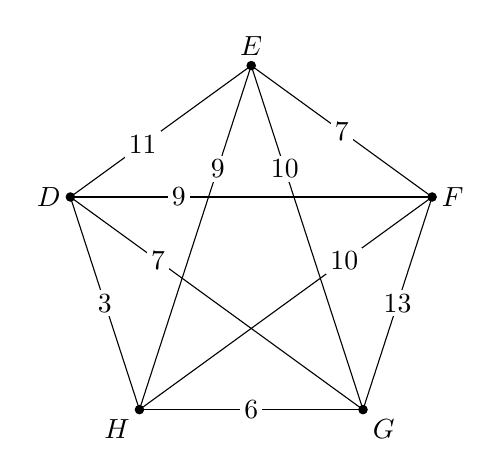
\begin{tikzpicture}[scale=1.15]
  \path (90:2.1) coordinate (E) (18:2.1) coordinate (F) (-54:2.1) coordinate (G) (-126:2.1) coordinate (H) (162:2.1) coordinate (D);
  \draw (D)--(E) node[pos=.4,fill=white,inner sep=1.5pt]{$11$};
  \draw (E)--(F) node[pos=.5,fill=white,inner sep=1.5pt]{$7$};
  \draw (F)--(G) node[pos=.5,fill=white,inner sep=1.5pt]{$13$};
  \draw (G)--(H) node[pos=.5,fill=white,inner sep=1.5pt]{$6$};
  \draw (H)--(D) node[pos=.5,fill=white,inner sep=1.5pt]{$3$};
  \draw (D)--(F) node[pos=.3,fill=white,inner sep=1.5pt]{$9$};
  \draw (E)--(H) node[pos=.3,fill=white,inner sep=1.5pt]{$9$};
  \draw (E)--(G) node[pos=.3,fill=white,inner sep=1.5pt]{$10$};
  \draw (F)--(H) node[pos=.3,fill=white,inner sep=1.5pt]{$10$};
  \draw (D)--(G) node[pos=.3,fill=white,inner sep=1.5pt]{$7$};
  \foreach \P in {D,E,F,G,H} \fill (\P) circle (1.5pt);
  \path (E) node[above]{$E$} (F) node[right]{$F$} (G) node[below right]{$G$} (H) node[below left]{$H$} (D) node[left]{$D$};
\end{tikzpicture}
\end{center}
\shortans{35}
\loigiai{Đường đi là một chu trình qua $D$ và $4$ hộp thư $E,F,G,H$, có $\dfrac{4!}{2}=12$ chu trình khác nhau (tính cả hai chiều là một).
Tổng thời gian của chúng lần lượt là: $DEFGHD=40$; $DEFHGD=41$; $DEGFHD=47$; $DEGHFD=46$; $DEHFGD=50$; $DEHGFD=48$; $DFEGHD=35$; $DFEHGD=38$; $DFGEHD=44$; $DFHEGD=45$; $DGEFHD=37$; $DGFEHD=39$.
Vậy thời gian ngắn nhất là $35$ phút, ứng với $D\to H\to G\to E\to F\to D$.}
\end{ex}
